% ============================================================================
\section{Parallel, flow, and diffusion acoustic models}
% ============================================================================

% --- Source: Ren et al.\ FastSpeech~2 (Works cited 9, 16); TTS Lecture Material Generation Request ---
\begin{frame}{FastSpeech 2: parallel mel generation}
  \begin{itemize}\footnotesize
    \item FastSpeech~2 uses a Feed-Forward Transformer (FFT) with a Length Regulator to match phoneme and spectrogram lengths, replacing soft attention.
    \item The Variance Adaptor predicts duration, pitch, and energy for more control over prosody.
    \item The Duration Predictor solves the "one-to-many" mapping, deciding exactly how many frames each phoneme lasts, which makes the system more stable.
    \item Pitch Predictor models the fundamental frequency ($F_0$); Energy Predictor models the loudness (from the spectrogram).
  \end{itemize}
  \centering
  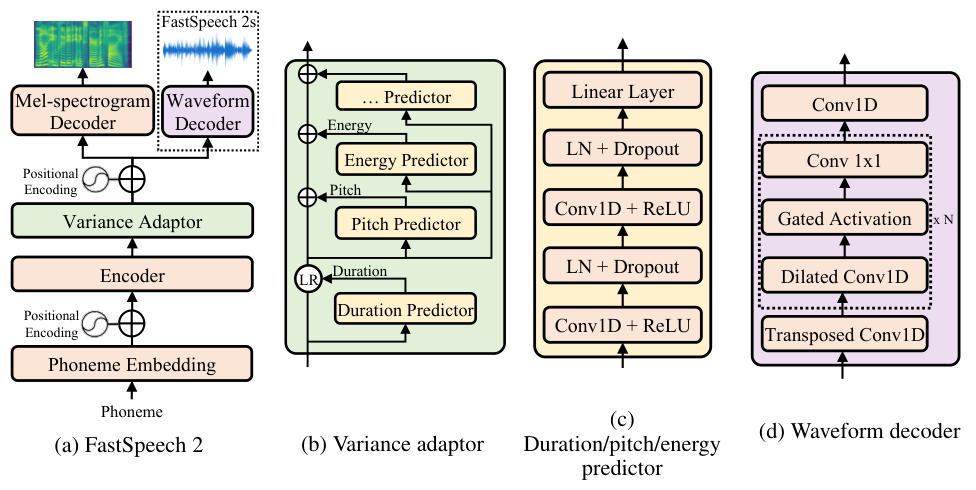
\includegraphics[width=0.92\textwidth,height=0.46\textheight,keepaspectratio]{assets/New-Lecture-TTS/fastspeech2_architecture_paper.png}
  \slideimgsource{Ren et al., ``FastSpeech 2: Fast and High-Quality End-to-End Text to Speech,'' Fig.~1(a); \href{https://arxiv.org/abs/2006.04558}{arXiv:2006.04558} (cropped).}
\end{frame}

% --- Source: Kim et al.\ Glow-TTS (Works cited 20, 22); TTS Lecture Material Generation Request ---
\begin{frame}{Glow-TTS and monotonic alignment search (MAS)}
  \begin{itemize}\footnotesize
    \item Glow-TTS uses Normalizing Flows to turn a simple distribution into a mel-spectrogram distribution.
    \item Monotonic Alignment Search (MAS) finds the single best monotonic path between text and speech using dynamic programming.
    \item Unlike soft attention, MAS avoids alignment breaks, so the model works well on long utterances.
  \end{itemize}
  \centering
  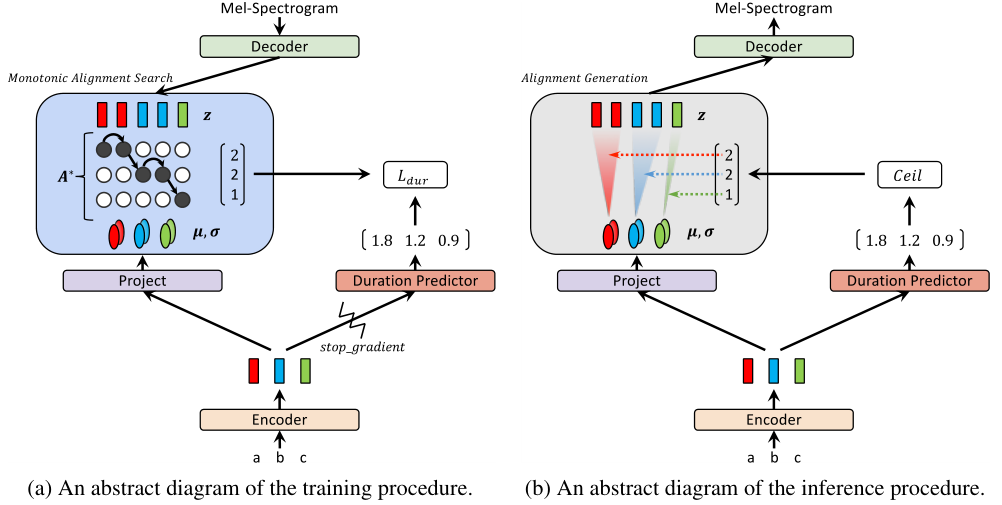
\includegraphics[width=0.90\textwidth,height=0.40\textheight,keepaspectratio]{assets/New-Lecture-TTS/glowtts_training_inference.png}
  \slideimgsource{Kim et al., ``Glow-TTS: A Generative Flow for Text-to-Speech via Monotonic Alignment Search,'' Fig.~1; \href{https://arxiv.org/abs/2005.11129}{arXiv:2005.11129}.}
\end{frame}

% --- Source: Popov et al.\ Grad-TTS (Works cited 21, 23--24); TTS Lecture Material Generation Request ---
\begin{frame}{Grad-TTS: diffusion in the acoustic domain}
  \begin{itemize}\footnotesize
    \item Grad-TTS uses score-based diffusion to turn random noise into structured mel-spectrograms.
    \item The reverse diffusion process is controlled by stochastic differential equations (SDEs).
    \item Users can control the trade-off between quality and speed by choosing the number of reverse steps.
    \item Grad-TTS can sound good with as few as 10 steps, and it is faster and more robust than Tacotron~2.
  \end{itemize}
  \centering
  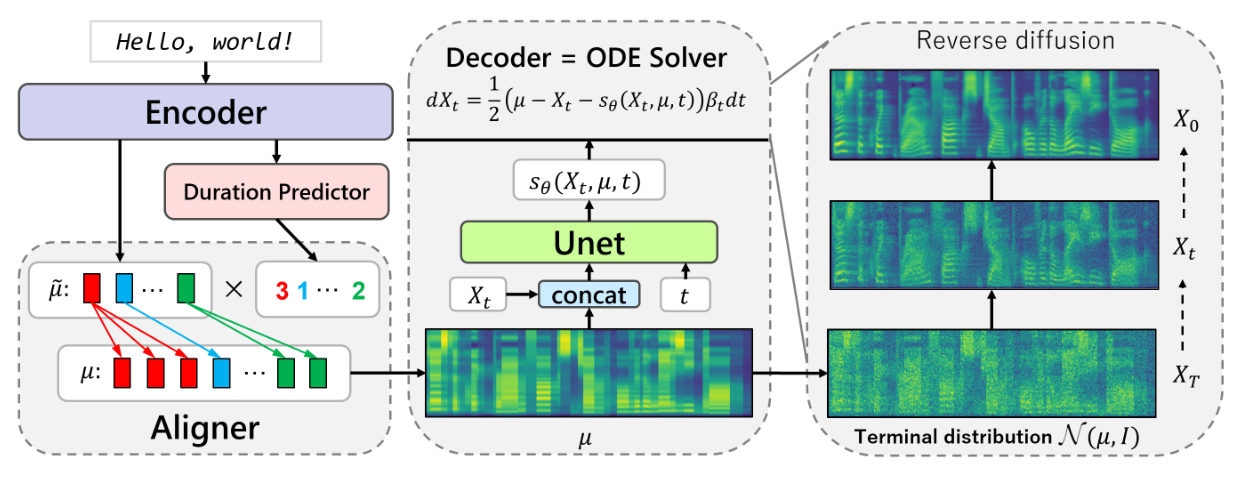
\includegraphics[width=0.95\textwidth,height=0.38\textheight,keepaspectratio]{assets/New-Lecture-TTS/gradtts_fig2_inference.png}
  \slideimgsource{Popov et al., ``Grad-TTS: A Diffusion Probabilistic Model for Text-to-Speech,'' Fig.~2; \href{https://arxiv.org/abs/2105.06337}{arXiv:2105.06337}.}
\end{frame}

\begin{frame}{HiFi-GAN and parallel front ends}
  \begin{itemize}\footnotesize
    \item HiFi-GAN is a GAN-based vocoder that can generate high-quality audio from mel-spectrograms.
    \item Parallel front ends like FastSpeech can generate mel-spectrograms in parallel, which is faster than sequential generation.
    \item The combination of FastSpeech and HiFi-GAN is a popular and effective way to synthesize speech.
  \end{itemize}
  \centering
  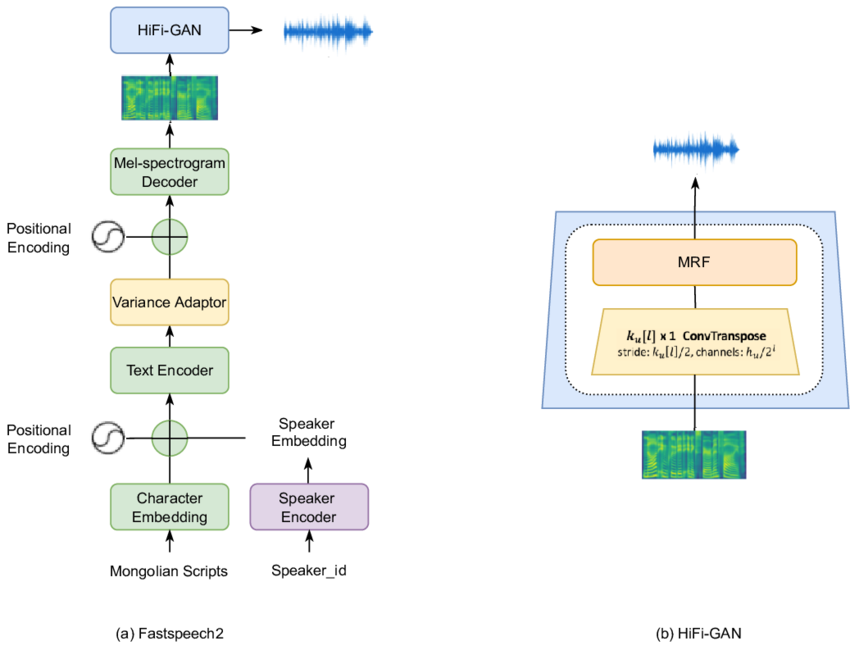
\includegraphics[width=\textwidth,height=0.52\textheight,keepaspectratio]{images/audio-nlp/fastspeech_hifigan.png}
  \slideimgsource{Kong et al., ``Generative Adversarial Networks for Efficient and High Fidelity Speech Synthesis,'' Fig.~1; \href{https://arxiv.org/abs/2010.05646}{arXiv:2010.05646}.}
\end{frame}

% --- Source: Kim, Kong, Son, VITS (arXiv:2106.06103), Fig.~1 ---
\begin{frame}{VITS: Variational Inference with Adversarial Learning for End-to-End Text-to-Speech}
  \begin{itemize}\footnotesize
    \item Connect two modules of TTS systems through latent variables to enable efficient end-to-end learning.
    \begin{itemize}
      \item generates more natural sounding audio than current two-stage models
    \end{itemize}
    \item At training: a posterior encoder reads real mels; monotonic alignment search (MAS) links text to speech; a discriminator improves waveform quality.
    \item At inference: text $\rightarrow$ text encoder + duration predictor $\rightarrow$ latent features $\rightarrow$ waveform decoder $\rightarrow$ audio (no separate vocoder).
  \end{itemize}
  \centering
  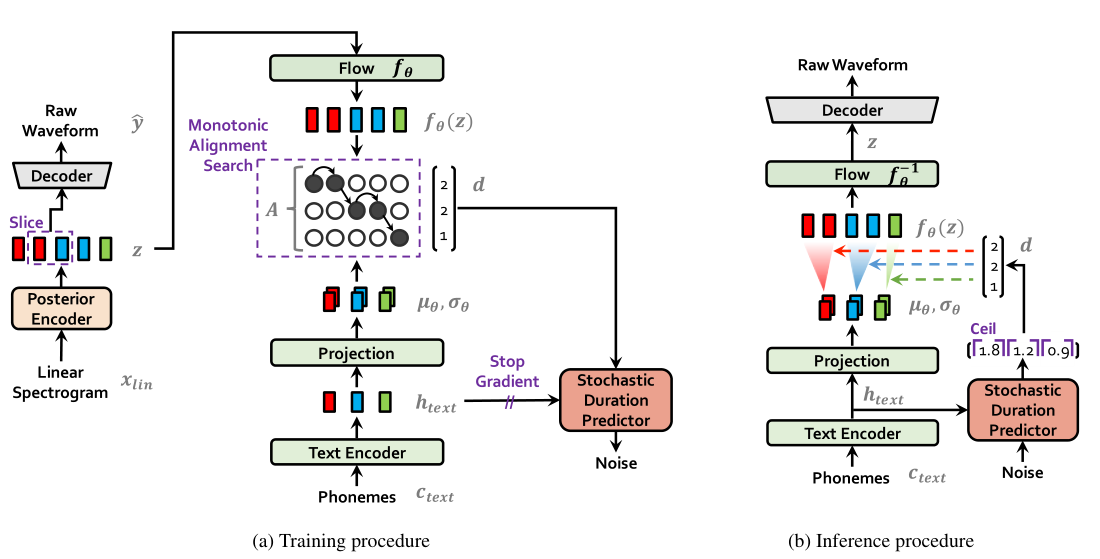
\includegraphics[width=0.98\textwidth,height=0.36\textheight,keepaspectratio]{assets/New-Lecture-TTS/vits_fig1_architecture.png}
  \slideimgsource{Kim, Kong, and Son, ``Conditional Variational Autoencoder with Adversarial Learning for End-to-End Text-to-Speech'' (VITS), Fig.~1; \href{https://arxiv.org/abs/2106.06103}{arXiv:2106.06103}.}
\end{frame}
